\documentclass[11pt]{article}

\usepackage[utf8]{inputenc}
\usepackage[T1]{fontenc}
\usepackage[margin=1in]{geometry}
\usepackage{microtype}
\usepackage{amsmath,amssymb}
\usepackage{booktabs}
\usepackage{array}
\usepackage{tabularx}
\usepackage{placeins}
\usepackage{graphicx}
\usepackage{xcolor}
\usepackage[numbers,sort&compress]{natbib}
\usepackage{caption}
\usepackage{enumitem}
\usepackage{xurl}
\usepackage{seqsplit}
\usepackage[colorlinks=true,linkcolor=blue!55!black,citecolor=blue!55!black,urlcolor=blue!55!black]{hyperref}

\emergencystretch=2.5em
\captionsetup{font=small,labelfont=bf}
\setlist[itemize]{leftmargin=1.5em,itemsep=0.22em}
\setlist[enumerate]{leftmargin=1.5em,itemsep=0.22em}

\newcommand{\codepath}[1]{\texttt{\nolinkurl{#1}}}
\newcommand{\codehash}[1]{{\ttfamily\small\seqsplit{#1}}}

\title{\textbf{Agentic Weight-Space Transplantation on Language Models}}

\author{Primary Investigator: Kaiwen Du}

\date{November 27, 2026}

\begin{document}

\maketitle

\vspace{-0.8em}
\begin{center}
\fbox{\parbox{0.96\linewidth}{\footnotesize
\textbf{Academic Research Scope Disclaimer:} This study is a non-commercial academic feasibility investigation operating exclusively on open-weight Apache-2.0 checkpoints (\texttt{Qwen/Qwen3.5-0.8B} and \texttt{Qwen/Qwen3.5-2B}). It does not perform knowledge distillation or develop models intended to compete with frontier model providers; automated editors operate strictly between pinned open-weight checkpoints. Repository freeze reference: \texttt{d12e8fb} (M3 evaluation \texttt{42b859b}, \texttt{H004} review \texttt{9c975e9}, Milestone M4).
}}
\end{center}
\vspace{0.3em}

\begin{abstract}
Weight-Space Programming (WSP) has shown that frontier language models can inspect neural weights and construct bounded single-model edits, raising the question of whether agents can go further and \emph{transplant} learned capabilities across models of different scales without gradient-based training. We present a preregistered, controlled empirical feasibility study of \textbf{Agentic Weight-Space Transplantation (AWST)} targeting grade-school mathematical reasoning from a stronger donor (\texttt{Qwen/Qwen3.5-2B}, 2.27B stored parameters) into a fixed-architecture smaller recipient (\texttt{Qwen/Qwen3.5-0.8B}, 873,438,784 stored parameters, 852,985,920 active runtime parameters, vision encoder strictly frozen across 153 tensors). We separate \textbf{weights-only transplantation (\texttt{T1})}, restricted to static donor tensor slices without donor forward passes, from \textbf{activation-assisted transplantation (\texttt{T2})}, which permits bounded donor probing on development prompts. To isolate genuine donor mathematical transfer from confounding mechanisms, we evaluate against unmodified baselines (\texttt{C0\_raw}, plus loop-repaired Stage~0 reference \texttt{C0\_loopfixed}), donor-free WSP (\texttt{C1}), random recipient perturbations (\texttt{C2}), unaligned donor slice copying (\texttt{C3}), conventional algorithmic transfer (\texttt{C4\_weights} via Procrustes + neuron matching; \texttt{C4\_act} via activation-guided pruning + ridge basis alignment), and shape- and norm-matched shuffled-donor controls (\texttt{C5}).

Under a frozen greedy, no-thinking, 1,024-token protocol (\texttt{enable\_thinking=False}) that eliminates 0.8B reasoning-loop confounds while preserving a large donor lead (+21.5 percentage points [pp] on isolated GSM8K and +44.0 pp on multi-digit carry arithmetic), neither frozen Stage~1 checkpoint (\texttt{T1} editing 9,050 tied digit-embedding entries; \texttt{T2} editing 2 Gated DeltaNet decay scalars) met the preregistered joint success criteria in isolated confirmatory evaluation ($n=200$ GSM8K, $n=150$ synthetic arithmetic, $n=100$ out-of-distribution [OOD] templates). On isolated GSM8K, \texttt{T1} scored 54.5\% versus 51.5\% for \texttt{C0\_raw} (+3.0 pp, 95\% bootstrap CI [$-$2.0, +8.0], exact McNemar $p = 0.345$), failing to exceed \texttt{C1} (+1.5 pp [$-$3.5, +6.5], Holm $p = 0.701$), \texttt{C4\_weights} (+7.5 pp [+1.0, +14.0], Holm $p = 0.080$), or shuffled-donor \texttt{C5\_T1\_rowperm} (+0.5 pp [$-$3.5, +4.5], $p = 1.000$). On the same test set, \texttt{T2} scored 51.5\% (0.0 pp [$-$3.5, +3.5] vs.\ \texttt{C0\_raw}, $p = 1.000$; $-$3.5 pp [$-$8.5, +1.0] vs.\ \texttt{C5\_T2\_norm\_matched}, $p = 0.230$) and dropped $-$5.0 pp [$-$10.0, $-$1.0] ($p = 0.0625$) on OOD problems. Whereas \texttt{T2}'s item-level interval on GSM8K excludes the +5.0 pp target for the evaluated checkpoint, \texttt{T1}'s interval still spans +5.0 pp and captures a single frozen editing session ($N=1$ per track), yielding a negative outcome on the joint criteria rather than proof of an exact zero effect for \texttt{T1}. In contrast, random unaligned donor copying (\texttt{C3}) suffered a $-$20.0 pp [$-$29.0, $-$11.0] OOD collapse ($p = 3.59\times 10^{-5}$) and degraded 10-passage prose perplexity (62.63 $\rightarrow$ 78.87), while aligned or ultra-sparse interventions avoided that specific drop. Finally, an HTTP 206 Byte-Range Safetensors reader reproduced target tensor slices bit-for-bit using 176,584 of 1,746,942,600 shard bytes (9,892.98$\times$ reduction). All Stage~0--1 local experiments and M3 confirmatory evaluations incurred \$0.00 in direct API/cloud charges (\$14.2912 cumulative Codex shadow cost across \texttt{H001}--\texttt{H004} within the \$20.00 M2 pilot gate); Stages~2--4 were formally skipped following Stage~1 failure.

\medskip
\noindent\textbf{Keywords:} weight-space programming, model merging, training-free knowledge transfer, mechanistic interpretability, mathematical reasoning, Gated DeltaNet
\end{abstract}

\section{Introduction}

Transferring specialized capabilities from large pretrained language models into compact on-device models ordinarily requires gradient-based fine-tuning, knowledge distillation, or large-scale activation-driven pruning and merging~\cite{fan2026apm,cui2026transport}. Recent work on \textbf{Weight-Space Programming (WSP)} demonstrates that frontier reasoning models can directly inspect serialized weight matrices, write interpretable weight programs, and execute surgical parameter edits that alter downstream behavior~\cite{takehi2026sparks,li2026weightcode}. In the motivating case study, Takehi et al.~\cite{takehi2026sparks} reported raising \texttt{Qwen3.5-0.8B} GSM8K accuracy from 13.8\% to 67.1\% by subtracting a single vector direction across 131,072 MLP entries (0.016\% of parameters).

Yet single-model WSP repairs primarily \emph{unblock} latent capabilities by suppressing repetitive reasoning loops rather than importing missing circuits~\cite{takehi2026sparks}. Moreover, follow-up replication work warns that frontier LLMs succeed most reliably when reading or writing shallow input-layer representations rather than deep internal algorithms~\cite{goworek2026replicating}, and that standard empirically risk-minimized (ERM) checkpoints are often brittle under direct weight perturbation unless trained specifically for editability~\cite{ropinski2026editready}. Whether an autonomous AI programmer can extend WSP across model boundaries---identifying a stronger capability in a larger \emph{donor} checkpoint, resolving hidden-dimension and basis mismatches, and transplanting that capability into a \emph{recipient} without gradient descent---remains untested under rigorous controls.

We formulate \textbf{Agentic Weight-Space Transplantation (AWST)} and investigate six research questions:

\begin{itemize}
\item \textbf{RQ1 (Primary feasibility):} Can an AI agent selectively identify, adapt, and transplant grade-school mathematical reasoning from a larger donor (\codepath{Qwen/Qwen3.5-2B}~\cite{qwen2026qwen35_2b}) into a smaller fixed-architecture recipient (\codepath{Qwen/Qwen3.5-0.8B}~\cite{qwen2026qwen35_08b}) without gradient-based training?
\item \textbf{RQ2 (Agent vs.\ algorithm):} Does agent-directed transplantation (\texttt{T1}, \texttt{T2}) outperform matched conventional algorithmic transfer (\texttt{C4\_weights}, \texttt{C4\_act})?
\item \textbf{RQ3 (Donor vs.\ self-repair):} Does donor access outperform donor-free agent weight editing of the recipient alone (\texttt{C1})?
\item \textbf{RQ4 (Cross-family generalization, gated):} Can AWST transfer across distinct model families (e.g., \codepath{Qwen/Qwen3.5-9B}~\cite{qwen2026qwen35_9b} $\rightarrow$ \codepath{google/gemma-4-E2B-it}~\cite{google2026gemma4e2b})? \emph{(Formally skipped under Decision \texttt{D011} after Stage~1 failed gate criteria.)}
\item \textbf{RQ5 (Selective remote weight access):} Can bounded HTTP 206 range retrieval read and verify target donor slices without downloading full multi-gigabyte shards (as a prerequisite for large MoE donors such as \codepath{moonshotai/Kimi-K3.1-Pro}~\cite{moonshot2026kimik31pro})?
\item \textbf{RQ6 (Exploratory agent comparison):} How do permitted harnesses (\texttt{GPT-6.2 Astra} vs.\ \texttt{Gemini 4 Neon}) compare on a controlled synthetic weight-space competency suite?
\end{itemize}

These questions map to a primary hypothesis (\textbf{H1}: \texttt{T1} or \texttt{T2} outperforms both \texttt{C1} and \texttt{C4} while meeting $\ge +5$ pp gain over \texttt{C0\_raw}, donor dependence over \texttt{C5}, OOD transfer, $\le 3$ pp retention loss, and unchanged architecture), competing against the null (\textbf{H0}), alongside secondary hypotheses testing unseen/non-loop generalization (\textbf{H2}), alignment against unaligned copying (\textbf{H3}), and byte-reduced selective remote access (\textbf{H4}).

\paragraph{Contributions and Honest Scoping.}
This study provides: (1) a preregistered experimental and statistical protocol separating weights-only (\texttt{T1}) and activation-assisted (\texttt{T2}) AWST tracks from reasoning-loop confounds, matched controls (\texttt{C0}--\texttt{C5}), and external hidden test sets; (2) an empirical Stage~1 evaluation showing that neither frozen \texttt{T1} (10 tied digit embeddings via ridge anchor mapping) nor \texttt{T2} (2 Gated DeltaNet decay scalars via activation routing and ablation) improved held-out math performance over unedited or shuffled-donor controls, exposing a sharp development-to-validation generalization mirage; (3) evidence supporting secondary hypotheses \textbf{H3} (unaligned \texttt{C3} suffers $-$20.0 pp OOD and +16.2 perplexity collapse) and \textbf{H4} (9,892.98$\times$ byte reduction via verified HTTP 206 reads); and (4) an open, auditable failure analysis incorporating an independent \texttt{H004} statistical review. Because Stage~1 evaluated one frozen session ($N=1$) per agent track and Stages~2--4 were stopped cleanly at the Stage~2 gate (\texttt{D011}), our findings provide negative feasibility evidence for these concrete single-session AWST strategies rather than proving impossibility across all future multi-session or dense subspace methods.

\section{Related Work}

\paragraph{Weight-Space Programming and Verification.}
Takehi et al.~\cite{takehi2026sparks} introduced Weight-Space Programming (WSP), showing GPT-6 Astra could write small policy networks and locate loop-inducing MLP directions in \texttt{Qwen3.5-0.8B} via bounded slice inspection and development forward passes, while noting cross-model circuit grafting as future work. Concurrent studies sharpen both the promise and boundaries of WSP. \emph{WeightCode}~\cite{li2026weightcode} shows LLMs can synthesize reusable closed-form weight-editing programs conditioned on task demonstrations, though cross-seed transfer was examined only within identical architectures. Goworek et al.~\cite{goworek2026replicating} replicate WSP on synthetic tasks and show that LLM weight reading relies heavily on decoding input-layer weight patterns rather than mechanistic comprehension of deeper circuits---a direct warning for weights-only transplantation (\texttt{T1}). Ropinski and Kranz~\cite{ropinski2026editready} find that standard ERM vision networks resist direct LLM edits unless pretrained with \emph{Edit-Ready Training}, and Gross~\cite{gross2026wspverify} combines WSP with formal verification to detect policy regressions. AWST operationalizes non-training verification via bit-exact structural invariants, \texttt{float64} reversion tests, and held-out retention suites.

\paragraph{Training-Free Model Merging and Cross-Scale Transfer.}
Independently trained networks occupy distinct coordinate bases and permutation symmetries, causing naive averaging or index-matched slicing to degrade performance unless neurons are aligned by weights or activations, as shown in \emph{Git Re-Basin}~\cite{ainsworth2023gitrebasin} and \emph{ZipIt!}~\cite{stoica2024zipit}. Extending to heterogeneous widths and architectures without gradient training, \emph{Activation-Prune-Merge (APM)}~\cite{fan2026apm} prunes salient donor dimensions from task-conditioned activation maps and merges them into smaller recipients, while \emph{Transport and Merge}~\cite{cui2026transport} computes neuron correspondences across distinct architectures via Optimal Transport over calibration activations. Consequently, training-free cross-scale transfer is not novel by itself; rather, AWST tests whether \emph{agent-directed} inspection and closed-form adaptation can match or surpass algorithmic alignment baselines (\texttt{C4}) while preserving donor-specific utility (\texttt{T1}/\texttt{T2} $>$ \texttt{C5}).

\paragraph{Safetensors Remote Metadata Parsing.}
Hugging Face~\cite{huggingface2026safetensors} documents inspecting Safetensors tensor headers via HTTP \texttt{Range} requests (\texttt{bytes=0-7} length prefix followed by JSON metadata). AWST evaluates whether exact HTTP 206 byte-range fetching can materialize isolated weight tensors cleanly (\textbf{H4}) without downloading entire multi-gigabyte checkpoints.

\section{Method}

\subsection{Operational Definitions and Track Separation}

Following our frozen protocol (\codepath{AWST_Research_Protocol_v0.3.md}, Section~4), we define the components of AWST:
\begin{itemize}
\item \textbf{Donor (\codepath{Qwen/Qwen3.5-2B}):} Pretrained open-weight checkpoint demonstrating superior mathematical reasoning (+21.5 pp isolated GSM8K lead over recipient).
\item \textbf{Recipient (\codepath{Qwen/Qwen3.5-0.8B}):} Smaller fixed-architecture checkpoint whose existing parameter tensors may be updated into derived directories without changing parameter count (873,438,784 stored entries), tensor shapes, layer count (24 text layers), tokenizer, or runtime graph, and with 0 gradient/backpropagation steps.
\item \textbf{Weights-Only Track (\texttt{T1}):} The editing agent may inspect donor and recipient checkpoint metadata, statistics, and bounded tensor slices ($\le 200$ MB payload cap) and run recipient forward passes on \codepath{data/development/}, but executes \textbf{zero donor forward passes} (\texttt{donor\_forward\_passes = 0}).
\item \textbf{Activation-Assisted Track (\texttt{T2}):} A strictly unpooled track permitting bounded donor forward passes ($\le 64$ prompts) on \codepath{data/development/} alongside weight inspection. Tracks \texttt{T1} and \texttt{T2} are logged under separate manifests (\texttt{H002}, \texttt{H003}), run in distinct Codex sessions, and analyzed against track-matched controls (\texttt{C4\_weights} vs.\ \texttt{C4\_act}).
\end{itemize}

\subsection{Agent Interface and Immutable Provenance}

Agents operate through a bounded Python toolbox (\texttt{AgentWeightToolbox} in \codepath{src/agent_interface/tools.py}) enforcing byte-read budgets, forward-pass counters, and tensor-size limits so raw multi-million-entry matrices are never serialized into prompt context. Every patch goes through \texttt{apply\_tensor\_patches} (\codepath{src/interventions/patch_applier.py}), writing derived \texttt{.safetensors} shards without mutating cached donor or recipient checkpoints, verifying exact total parameter counts, dtype preservation, and bit-exact SHA-256 invariance across all 153 multimodal vision tensors (\codepath{model.visual.*} / \codepath{visual.*}, per \texttt{D003}). Independent verification scripts (\texttt{verify\_h002.py}, \texttt{verify\_h003.py}) enforce full-shard deterministic CLI replay and \texttt{float64} delta subtraction restoring the pristine recipient shard SHA-256 with zero differing parameters.

\subsection{Implemented Interventions and Control Arms}

All 10 arms evaluated in M3 (plus \texttt{C2} validation reference and \texttt{C0\_loopfixed} Stage~0 reference) are deterministic functions of pinned checkpoints and \codepath{data/development/}:

\begin{enumerate}
\item \textbf{\texttt{C0\_raw} (Unmodified Recipient):} Pinned \codepath{Qwen/Qwen3.5-0.8B} (\texttt{2fc06364...}) evaluated without modification. Stage~0 also verified \texttt{C0\_loopfixed}, applying Takehi et al.'s~\cite{takehi2026sparks} \texttt{p50c} direction across 130,188 \texttt{bfloat16} entries in layers 15 and 19 \codepath{mlp.down_proj.weight} (\texttt{rel\_frob = 0.002379}).
\item \textbf{\texttt{C1} (Donor-Free Agent WSP, \texttt{H002}):} Edits strictly the 10 individual ASCII digit rows (token IDs 15--24, corresponding to digits \texttt{0}--\texttt{9}) in \codepath{model.language_model.embed_tokens.weight} (tied to LM head) to expand between-digit contrast away from the 10-digit centroid. Letting $R \in \mathbb{R}^{10 \times 1024}$ denote the digit rows and $Z = R - \bar{R}$, \texttt{C1} writes $\operatorname{BF16}(R + a Z)$ with screen-selected radius $a = 1/32$ chosen prior to opening any donor tensor (9,097 changed entries, overall relative Frobenius norm $3.961\times 10^{-5}$).
\item \textbf{\texttt{T1} (Weights-Only AWST, \texttt{H002}):} Inspects only the 10 digit rows and 30 fixed arithmetic anchor rows (spelled digits, arithmetic operators, and spaced math words; token IDs verified identical across 2B and 0.8B) with 0 donor forward passes. Let $A_d \in \mathbb{R}^{30 \times 2048}$ and $A_r \in \mathbb{R}^{30 \times 1024}$ be centered, row-normalized anchor matrices, and $C = Z A^\top / \|Z\|_F \in \mathbb{R}^{10 \times 30}$ denote normalized digit-to-anchor similarity tables. Solving the 30-dimensional ridge system in \texttt{float64}:
\begin{equation}
F = \operatorname{center\_rows}\!\left((C_d - C_r)\left(A_r A_r^\top + \frac{1}{8} I\right)^{-1} A_r\right), \quad
R' = \operatorname{BF16}\!\left(R_r + a \|Z_r\|_F \frac{F}{\|F\|_F}\right)
\end{equation}
transfers relative donor digit-anchor geometry into the recipient's native embedding basis. Screening selected radius $a = 1/32$ over $1/8$ (9,050 changed entries, \texttt{rel\_frob} $= 3.953\times 10^{-5}$). Although anchor alignment error $\|C_d - C_r\|_F$ dropped from 0.18545 to 0.15158 at $a=1/32$ and 0.05412 at $a=1/8$, the stronger radius scored lower on the 40-item dev screen (17/40 vs.\ 19/40).
\item \textbf{\texttt{T2} (Activation-Assisted AWST, \texttt{H003}):} Uses 56/64 allowed donor forward passes (16 carry + 16 GSM8K prompts for routing/prefill probes plus 24 prompts for two shortlisted head ablations) across the 12 mid-to-late Gated DeltaNet layers (\texttt{layers 8..23} linear attention heads). Correlation of write gate and log-decay magnitude plus numeric-token RMS selectivity shortlisted (layer~14, head~5) and (layer~13, head~12); signed ablation gap (donor minus recipient drop) selected \textbf{Layer~13, Head~12}. Notably, donor margin slightly \emph{increased} (+0.0208 on 6 GSM8K probes, 0.0 on 6 carry probes) under L13 H12 ablation, providing little causal evidence of head necessity. \texttt{T2} modifies two recurrent decay scalars at head index 12---\codepath{layers.13.linear_attn.A_log} (\texttt{float32}) and \codepath{dt_bias} (\texttt{bfloat16})---via $\operatorname{cast}(r + s \cdot (\text{target} - r))$ using donor scalar values plus a median numeric-token decay offset (+0.0641682148). Dev screening selected strength $s = 0.5$ over 1.0 (2 changed parameters, \texttt{rel\_frob} $= 1.769\times 10^{-4}$, shifting estimated isolated memory half-life from 26.66 to 26.22 token steps vs.\ 25.76 for the donor).
\item \textbf{\texttt{C4\_weights} (Conventional Weights-Only Baseline):} Orthogonal Procrustes alignment $P \in \mathbb{R}^{2048 \times 1024}$ computed from SVD of 16,384 shared embedding rows ($E_d^\top E_r$), followed by weights-only salience pruning ($6144 \rightarrow 3584$ MLP neurons via $\|\text{gate}\| \|\text{up}\| \|\text{down}\|$ product), Hungarian cosine neuron assignment (\codepath{scipy.optimize.linear_sum_assignment}), norm-matching, and dense SwiGLU interpolation ($\alpha = 0.05$) across layers 8--23 (48 tensors, 172,514,552 params, \texttt{rel\_frob} $= 1.003\times 10^{-2}$).
\item \textbf{\texttt{C4\_act} (Conventional Activation-Assisted Baseline):} Uses 32 development prompts (16 carry + 16 GSM8K) to solve ridge input/output projections ($\lambda = 10^{-2}$) and rank donor neurons by mean absolute intermediate activation plus cross-model correlation for Hungarian matching across layers 8--23 MLPs ($\alpha = 0.02$, 48 tensors, 168,325,062 params, \texttt{rel\_frob} $= 4.409\times 10^{-3}$).
\item \textbf{\texttt{C2} (Random Recipient Noise, Validation Reference):} Gaussian MLP perturbations across layers 8--23 matched to \texttt{C4\_weights} per-tensor relative norm (\texttt{rel\_frob} $= 1.019\times 10^{-2}$, 171,469,128 params).
\item \textbf{\texttt{C3} (Random Unaligned Donor Slice):} Copies random unaligned index subsets from donor layers 8--23 MLPs, matches Frobenius norm to recipient, and interpolates at $\alpha = 0.05$ (173,198,193 params, \texttt{rel\_frob} $= 1.116\times 10^{-2}$).
\item \textbf{\texttt{C5} (Shuffled-Donor Controls):} Applies the \emph{identical} \texttt{apply\_t1} (\texttt{C5\_T1\_rowperm}, permuting \codepath{embed_tokens.weight} rows with \texttt{seed=42}, 9,058 changed params, \texttt{rel\_frob} $= 3.945\times 10^{-5}$, cosine similarity $-$0.003 with \texttt{T1}) and \texttt{apply\_t2} (\texttt{C5\_T2\_perm} at 13.32$\times$ norm and \texttt{C5\_T2\_norm\_matched} rescaled to 0.985$\times$ of \texttt{T2}'s norm, 2 changed params, \texttt{rel\_frob} $= 1.743\times 10^{-4}$, cosine $-$0.765 with \texttt{T2}). Crucially, \texttt{C5\_T2\_norm\_matched} conditions on \texttt{T2}'s activation-localized (L13, H12) slot and offset, specifically testing dependence on authentic donor scalar values versus arbitrary perturbations at that locus.
\end{enumerate}

\subsection{Remote Selective Safetensors Retrieval (\textbf{H4})}

To test weights-only retrieval feasibility without full shard downloads (\codepath{src/weight_io/remote_range.py}), we built a strict HTTP \texttt{Range} client performing an initial 8-byte header-length read (\texttt{bytes=0-7}), a bounded metadata header read (\texttt{bytes=8-59847}), and exact tensor byte-span fetches validated for HTTP 206 Partial Content and matching \texttt{Content-Range} headers (aborting any unexpected HTTP 200 full-body response), backed by a byte-budgeted local chunk cache.

\section{Experimental Setup}

\paragraph{Harness Roles and Workflow Isolation.}
Research coordination, evaluation infrastructure, baseline and control implementations (\texttt{C0}, \texttt{C2}, \texttt{C3}, \texttt{C4}, \texttt{C5}), and independent replay/statistical verification were executed in Google Antigravity (\texttt{Gemini 4 Neon}), while Stage~1 weight transplantation trials (\texttt{H002} and \texttt{H003}) and the independent M3 statistical review (\texttt{H004}) were performed by Codex (\texttt{GPT-6.2 Astra}) via self-contained researcher-mediated manual handoffs under frozen development-only visibility and separate track manifests.

\paragraph{Checkpoints, Hardware, and Runtime Stack.}
Experiments ran locally on an Apple M4 Max (36 GiB unified memory, 14 CPU cores, macOS 27.2.1) using a pinned Python 3.11.16 environment (\texttt{torch 2.15.0} MPS \texttt{bfloat16}, \texttt{transformers 5.24.1}, \texttt{safetensors 0.8.0}, \texttt{datasets 5.2.0}, \texttt{scipy}) consuming 18 GB total local cache ($< 30$ GB cap). Checkpoints were pinned by exact Hugging Face revision: \codepath{Qwen/Qwen3.5-0.8B} (revision \codehash{2fc06364715b967f1860aea9cf38778875588b17}, primary shard SHA-256 \codehash{04b1c301...}) and \codepath{Qwen/Qwen3.5-2B} (revision \codehash{15852e8c16360a2fea060d615a32b45270f8a8fc}, primary shard SHA-256 \codehash{aa33250c...}). Both share 24 text layers (3:1 Gated DeltaNet + Full Attention, \texttt{head\_dim=256}, \texttt{vocab\_size=248320}, tied embeddings), differing in \texttt{hidden\_size} (1024 vs.\ 2048) and \texttt{intermediate\_size} (3584 vs.\ 6144). Inspection revealed that serialized checkpoints contain 488 tensors (873,438,784 entries), whereas \texttt{Transformers} instantiates 473 runtime parameters (852,985,920 entries), omitting 15 multi-token-prediction (\texttt{mtp.*}, 20,452,864 entries) tensors; both counts were verified on patch save/reload.

\paragraph{Stage 0 Protocol Calibration (\texttt{D002}).}
Evaluating \texttt{enable\_thinking=True} (\texttt{max\_new\_tokens=2048}, \texttt{temp=0.6}, \texttt{top\_p=0.95}, \texttt{top\_k=20}, without vLLM \texttt{presence\_penalty=1.5} or 32K context) reproduced severe 0.8B looping (95.0\% $\rightarrow$ 75.0\% with \texttt{C0\_loopfixed}, 25.0\% $\rightarrow$ 30.0\% GSM8K $n=20$, 100\% truncated). By contrast, freezing \texttt{enable\_thinking=False}, greedy decoding (\texttt{do\_sample=False}), and \texttt{max\_new\_tokens=1024} reduced \texttt{C0\_raw} GSM8K loops to 2.0\%, yielded 62.0\% GSM8K validation accuracy (outperforming \texttt{C0\_loopfixed}'s 56.0\%), ran $\sim 5\times$ faster (109.4 tok/s), and preserved large donor gaps (+20.0 pp GSM8K, +38.0 pp \texttt{carry\_add\_sub}). We therefore froze \texttt{nothink 1024} greedy on \texttt{C0\_raw} in Pilot Protocol v1.0 (\codepath{docs/preregistration.md}).

\paragraph{Datasets and Physical Test Isolation.}
Synthetic arithmetic (\codepath{src/data/synthetic_arithmetic.py}) spans three graded sub-skills (\texttt{carry\_add\_sub}: 3--5 digit add/subtract with $\ge 2$ carries/borrows; \texttt{mult\_2x2\_3x1}; \texttt{word\_2step}) alongside 6 disjoint held-out OOD phrasing templates (\texttt{synthetic\_ood\_test}, $n=100$). Public GSM8K splits used official training items for dev/val (500/200). Prior to opening the external test directory (\codepath{/Users/kaiwendu/.awst_isolated_eval/}), commit \texttt{d12e8fb} froze all 10 checkpoints and the M3 evaluation matrix (\texttt{D011} [originally \texttt{D010} at freeze], \codepath{runs/manifests/m3_frozen_checkpoint_audit.json}): seeded \texttt{gsm8k\_test} ($n=200$, \texttt{Random(20261126)} from 1,319), balanced \texttt{synthetic\_test} ($n=150$, 50/subskill), full \texttt{synthetic\_ood\_test} ($n=100$), a 30-item non-math IFEval-style format suite (\texttt{retention.py}, 6 constraint categories $\times$ 5 items), and teacher-forced perplexity across 10 original non-math English passages (557 predicted tokens). Raw isolated model completions reside exclusively outside the repository at \codepath{/Users/kaiwendu/.awst_isolated_eval/m3_logs/}.

\paragraph{Parsing and Statistical Analysis.}
Answers are extracted deterministically (\codepath{src/evaluation/parser.py}) checking \verb|\boxed{...}|, \texttt{\#\#\#\# ...}, \texttt{"final answer is/:"}, and a last-number fallback, alongside truncation ($\ge 1024$ tokens) and heuristic $n$-gram loop diagnostics. Paired comparisons compute exact percentage-point differences, 10,000-resample paired bootstrap 95\% confidence intervals (\texttt{default\_rng(42)}), exact two-sided McNemar binomial $p$-values, and separate per-track, per-endpoint Holm-Bonferroni adjustments (\{\texttt{T1} vs.\ \texttt{C1}, \texttt{T1} vs.\ \texttt{C4\_weights}\} and \{\texttt{T2} vs.\ \texttt{C1}, \texttt{T2} vs.\ \texttt{C4\_act}\}).

\section{Results}

\subsection{Stage 0 Reference, Remote Range Retrieval (\textbf{H4}), and RQ6 Competency}

\begin{table}[htbp]
\centering
\caption{Stage 0 calibration baselines, exploratory \texttt{RQ6} synthetic toy-network comparison (with disclosed aggregate-score visibility caveat before Astra's session), and M1 HTTP 206 selective Safetensors verification.}
\label{tab:stage0}
\setlength{\tabcolsep}{5pt}
\resizebox{\textwidth}{!}{%
\begin{tabular}{@{}lrrrl@{}}
\toprule
Evaluation / Metric & \texttt{C0\_raw} (0.8B) & \texttt{C0\_loopfixed} (\texttt{p50c}) & \texttt{Qwen3.5-2B} (Donor) & Notes / Reference \\
\midrule
\texttt{gsm8k\_val} ($n=100$, \texttt{nothink 1024}) & 62.0\% & 56.0\% & 82.0\% (+20.0 pp) & M1 baseline \\
\texttt{carry\_add\_sub} ($n=50$, \texttt{nothink 1024}) & 40.0\% & 30.0\% & 78.0\% (+38.0 pp) & Primary diagnostic (\texttt{D004}) \\
\texttt{mult\_2x2\_3x1} / \texttt{word\_2step} ($n=50$ ea.) & 68.0\% / 90.0\% & 62.0\% / 92.0\% & 86.0\% / 100.0\% & \texttt{word\_2step} at ceiling \\
\texttt{think 2048} GSM8K ($n=20$, no \texttt{pres\_pen}) & 25.0\% (95\% loop) & 30.0\% (75\% loop) & --- & Both 100\% trunc.\ (103--104 tok/s) \\
\texttt{RQ6} Toy Competency (Tasks A--C) & Neon: 3/3 (1.0 agr.) & Astra: 3/3 (1.0 agr.) & --- & Astra \$1.1003 shadow / \$0.00 API \\
HTTP 206 Retrieval (\texttt{Qwen 0.8B}) & 176,584 / 1,746,942,600 B & \textbf{9,892.98$\times$ red.} & \texttt{bit\_exact\_match: true} & \texttt{input\_layernorm} + \texttt{down\_proj} slice \\
\bottomrule
\end{tabular}}
\end{table}

Both \texttt{Gemini 4 Neon} and \texttt{GPT-6.2 Astra} achieved 3/3 (1.0 functional agreement) on the deterministic \texttt{RQ6} toy-network suite (weight construction, affine parameter recovery, and corruption localization) in single sessions, confirming tool literacy without predicting real-LLM transplantation outcomes (Table~\ref{tab:stage0}). Meanwhile, selective HTTP 206 reads reduced transferred bytes nearly four orders of magnitude (9,892.98$\times$, 1 cache hit) while matching local tensors bit-for-bit, positively establishing retrieval engineering feasibility (\textbf{H4} prerequisite).

\subsection{Development-to-Validation Generalization Mirage (M2 \texttt{H002} and \texttt{H003})}

During \codepath{data/development/} tuning, both Codex tracks appeared weakly promising on GSM8K: on the $n=480$ disjoint GSM8K development remainder, \texttt{T1} solved 273/480 (56.9\%) vs.\ 254/480 (52.9\%) for \texttt{C0\_raw} (+4.0 pp, 38 newly correct / 19 regressed) while slipping slightly on carry remainder (99/280 vs.\ 103/280, $-$1.4 pp); on the $n=64$ \texttt{H003} follow-up slice, \texttt{T2} solved 38/64 (59.4\%) vs.\ 36/64 (56.2\%) for \texttt{C0\_raw} (+3.1 pp [$-$3.1, +9.4]) and 27/64 (42.2\%) vs.\ 26/64 (40.6\%) on carry (+1.6 pp [$-$7.8, +10.9]).

On blinded \codepath{data/validation/} ($n=100$ GSM8K, $n=50$ carry/subskill), every gain disappeared (Figure~\ref{fig:split_trajectory}):
\begin{itemize}
\item \textbf{\texttt{T1} (\texttt{H002}):} 57.0\% GSM8K ($-$5.0 pp [$-$13.0, +2.0] vs.\ \texttt{C0\_raw} 62.0\%, $p = 0.302$) and 40.0\% carry (0.0 pp), trailing or matching \texttt{C1} (59.0\% / 36.0\%), \texttt{C4\_weights} (60.0\% / 40.0\%), \texttt{C5\_elem} (56.0\% / 32.0\%), and \texttt{C5\_rowperm} (59.0\% / 40.0\%).
\item \textbf{\texttt{T2} (\texttt{H003}):} 57.0\% GSM8K ($-$5.0 pp [$-$11.0, +1.0] vs.\ \texttt{C0\_raw}, $p = 0.180$) and 38.0\% carry ($-$2.0 pp), trailing or matching \texttt{C4\_act} (62.0\% / 34.0\%), \texttt{C5\_perm} (57.0\% / 34.0\%), and \texttt{C5\_norm\_matched} (59.0\% / 34.0\%). Meanwhile, \texttt{C2} scored 63.0\% / 36.0\% and \texttt{C3} dropped to 55.0\% GSM8K / 40.0\% carry.
\end{itemize}
Because Stage~1 showed zero held-out validation advantage, Stages~2 (\texttt{Qwen3.5-9B}), 3 (\texttt{Gemma 4 E2B}), and 4 (\texttt{Kimi K3.1 Pro}) were formally skipped (\texttt{D011}) prior to opening isolated evaluation.

\begin{figure}[htbp]
\centering
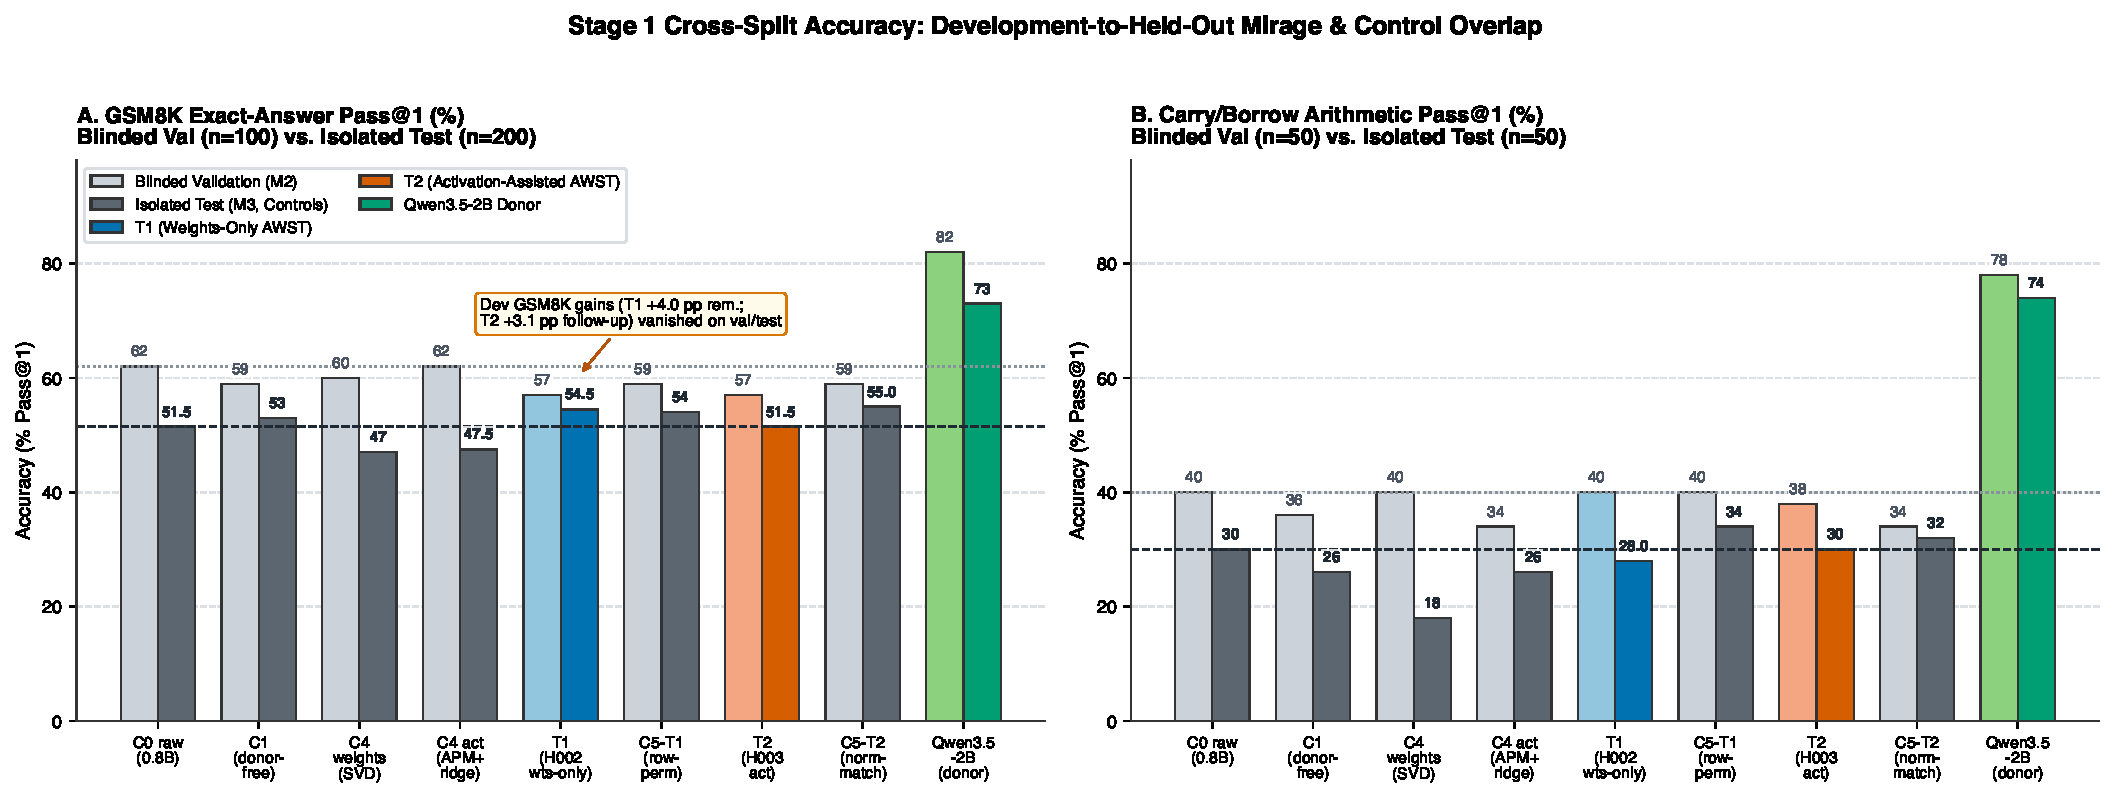
\includegraphics[width=\textwidth]{figures/fig1_split_trajectory.pdf}
\caption{GSM8K and carry/borrow pass@1 across blinded validation (M2) and isolated confirmatory test (M3). Development GSM8K gains for \texttt{T1} and \texttt{T2} failed to transfer, and both frozen AWST checkpoints overlapped unedited \texttt{C0\_raw} and shuffled-donor \texttt{C5} controls while \texttt{Qwen3.5-2B} maintained a +21.5 pp to +44.0 pp isolated lead.}
\label{fig:split_trajectory}
\end{figure}
\FloatBarrier

\subsection{Isolated Confirmatory Evaluation Scorecard (M3)}

In isolated confirmatory evaluation (Table~\ref{tab:m3_scorecard}, Table~\ref{tab:m3_contrasts}, Figures~\ref{fig:forest_contrasts} and~\ref{fig:edit_magnitude}), the donor model (\texttt{Qwen3.5-2B}) maintained a decisive lead over \texttt{C0\_raw} (+21.5 pp on \texttt{gsm8k\_test}, $p < 10^{-7}$; +44.0 pp on \texttt{carry\_add\_sub}, $p = 2.74\times 10^{-5}$). Across the nine 0.8B-architecture arms, neither \texttt{T1} (54.5\% GSM8K, 28.0\% carry, 77.0\% OOD) nor \texttt{T2} (51.5\% GSM8K, 30.0\% carry, 74.0\% OOD) outperformed donor-free \texttt{C1} (53.0\% GSM8K), algorithmic baselines \texttt{C4\_weights}/\texttt{C4\_act} after Holm correction ($p = 0.080$ and $p = 0.6635$), or shuffled-donor \texttt{C5} controls (54.0\% and 55.0\% GSM8K). Dense algorithmic transfer slightly degraded both GSM8K (47.0\% and 47.5\%) and prose perplexity (73.86 and 66.50 vs.\ 62.63 baseline), whereas unaligned random donor copying (\texttt{C3}) suffered a sharp $-$20.0 pp OOD failure ($p = 3.59\times 10^{-5}$) and rose to 78.87 prose perplexity.

\begin{table}[htbp]
\centering
\caption{M3 isolated 10-arm confirmatory scorecard (\texttt{nothink 1024} greedy, Apple M4 Max MPS \texttt{bfloat16}). All nine 0.8B-architecture arms verified identical 873,438,784 stored parameters, 153/153 frozen vision tensors, 2395.8 MB post-evaluation MPS driver allocation (4827.8 MB for 2B), 0.0\% GSM8K invalid parses, and 0 gradient steps.}
\label{tab:m3_scorecard}
\setlength{\tabcolsep}{4pt}
\resizebox{\textwidth}{!}{%
\begin{tabular}{@{}lrrrrrrrrr@{}}
\toprule
Arm & \texttt{gsm8k} ($n=200$) & \texttt{carry} ($n=50$) & \texttt{mult} ($n=50$) & \texttt{word} ($n=50$) & \texttt{ood} ($n=100$) & \texttt{ret\_ifeval} ($n=30$) & \texttt{prose\_ppl} & \texttt{tok/s} & Changed Params (\texttt{rel\_frob}) \\
\midrule
\texttt{C0\_raw} & 51.5\% & 30.0\% & 66.0\% & 96.0\% & 79.0\% & 70.0\% (21/30) & 62.63 & 106.5 & 0 (0) \\
\texttt{Qwen3.5-2B} & \textbf{73.0\%} & \textbf{74.0\%} & \textbf{86.0\%} & \textbf{100.0\%} & \textbf{81.0\%} & 66.7\% (20/30) & 41.02 & 61.3 & Reference donor \\
\texttt{C1} (1/32 centroid) & 53.0\% & 26.0\% & 64.0\% & 98.0\% & 78.0\% & 70.0\% (21/30) & 62.63 & 101.9 & 9,097 ($3.96\times 10^{-5}$) \\
\texttt{C3} (random 2B slice) & 49.5\% & 20.0\% & 60.0\% & 86.0\% & \textbf{59.0\%} & 66.7\% (20/30) & \textbf{78.87} & 102.5 & 173.20M ($1.12\times 10^{-2}$) \\
\texttt{C4\_weights} (SVD/Hung.) & 47.0\% & 18.0\% & 72.0\% & 90.0\% & 72.0\% & 63.3\% (19/30) & 73.86 & 106.9 & 172.51M ($1.00\times 10^{-2}$) \\
\texttt{C4\_act} (APM+ridge) & 47.5\% & 26.0\% & 68.0\% & 94.0\% & 79.0\% & 73.3\% (22/30) & 66.50 & 106.7 & 168.33M ($4.41\times 10^{-3}$) \\
\textbf{\texttt{T1} (\texttt{H002} wts-only)} & 54.5\% & 28.0\% & 66.0\% & 96.0\% & 77.0\% & 70.0\% (21/30) & 62.62 & 100.9 & 9,050 ($3.95\times 10^{-5}$) \\
\texttt{C5\_T1\_rowperm} & 54.0\% & 34.0\% & 62.0\% & 94.0\% & 79.0\% & 70.0\% (21/30) & 62.62 & 101.3 & 9,058 ($3.95\times 10^{-5}$) \\
\textbf{\texttt{T2} (\texttt{H003} act-assist.)} & 51.5\% & 30.0\% & 62.0\% & 98.0\% & 74.0\% & 70.0\% (21/30) & 62.47 & 101.4 & 2 ($1.77\times 10^{-4}$) \\
\texttt{C5\_T2\_norm\_matched} & 55.0\% & 32.0\% & 60.0\% & 96.0\% & 79.0\% & 70.0\% (21/30) & 62.61 & 101.6 & 2 ($1.74\times 10^{-4}$) \\
\bottomrule
\end{tabular}}
\end{table}

\begin{table}[htbp]
\centering
\caption{Paired M3 contrasts (10,000-resample bootstrap 95\% CIs, exact two-sided McNemar $p$, and track-isolated Holm-Bonferroni $p$). All 133 contrast-by-endpoint tables and 6 Holm families reproduced identically in independent audit \texttt{H004}.}
\label{tab:m3_contrasts}
\setlength{\tabcolsep}{5pt}
\resizebox{\textwidth}{!}{%
\begin{tabular}{@{}llrrrr@{}}
\toprule
Contrast ($B - A$) & Endpoint ($n$) & Gains / Losses & Diff (pp) [95\% Boot CI] & Exact McNemar $p$ & Track Holm $p$ \\
\midrule
\texttt{Qwen3.5-2B} $-$ \texttt{C0\_raw} & \texttt{gsm8k\_test} (200) & 52 / 9 & \textbf{+21.5} [+14.5, +28.5] & $< 10^{-7}$ & --- \\
\texttt{Qwen3.5-2B} $-$ \texttt{C0\_raw} & \texttt{carry\_add\_sub} (50) & 25 / 3 & \textbf{+44.0} [+26.0, +60.0] & 0.000027 & --- \\
\midrule
\texttt{T1} $-$ \texttt{C0\_raw} & \texttt{gsm8k\_test} (200) & 17 / 11 & +3.0 [$-$2.0, +8.0] & 0.3449 & --- \\
\texttt{T1} $-$ \texttt{C1} \emph{(primary)} & \texttt{gsm8k\_test} (200) & 15 / 12 & +1.5 [$-$3.5, +6.5] & 0.7011 & \textbf{0.7011} \\
\texttt{T1} $-$ \texttt{C4\_weights} \emph{(primary)} & \texttt{gsm8k\_test} (200) & 31 / 16 & +7.5 [+1.0, +14.0] & 0.0400 & \textbf{0.0800} \\
\texttt{T1} $-$ \texttt{C5\_T1\_rowperm} & \texttt{gsm8k\_test} (200) & 9 / 8 & +0.5 [$-$3.5, +4.5] & 1.0000 & --- \\
\texttt{T1} $-$ \texttt{C0\_raw} & \texttt{carry\_add\_sub} (50) & 2 / 3 & $-$2.0 [$-$10.0, +6.0] & 1.0000 & --- \\
\texttt{T1} $-$ \texttt{C0\_raw} & \texttt{synthetic\_ood} (100) & 4 / 6 & $-$2.0 [$-$8.0, +4.0] & 0.7539 & --- \\
\midrule
\texttt{T2} $-$ \texttt{C0\_raw} & \texttt{gsm8k\_test} (200) & 6 / 6 & 0.0 [$-$3.5, +3.5] & 1.0000 & --- \\
\texttt{T2} $-$ \texttt{C1} \emph{(primary)} & \texttt{gsm8k\_test} (200) & 14 / 17 & $-$1.5 [$-$7.0, +4.0] & 0.7201 & \textbf{0.7201} \\
\texttt{T2} $-$ \texttt{C4\_act} \emph{(primary)} & \texttt{gsm8k\_test} (200) & 30 / 22 & +4.0 [$-$3.0, +11.0] & 0.3317 & \textbf{0.6635} \\
\texttt{T2} $-$ \texttt{C5\_T2\_norm\_matched} & \texttt{gsm8k\_test} (200) & 9 / 16 & $-$3.5 [$-$8.5, +1.0] & 0.2295 & --- \\
\texttt{T2} $-$ \texttt{C0\_raw} & \texttt{synthetic\_ood} (100) & 0 / 5 & $-$5.0 [$-$10.0, $-$1.0] & 0.0625 & --- \\
\midrule
\texttt{C3} $-$ \texttt{C0\_raw} (\textbf{H3} failure) & \texttt{synthetic\_ood} (100) & 2 / 22 & \textbf{$-$20.0} [$-$29.0, $-$11.0] & \textbf{0.000036} & --- \\
\texttt{C4\_weights} $-$ \texttt{C3} (\textbf{H3} closest) & \texttt{synthetic\_ood} (100) & 20 / 7 & +13.0 [+3.0, +23.0] & 0.0192 & --- \\
\texttt{C4\_act} $-$ \texttt{C3} (\textbf{H3}) & \texttt{synthetic\_ood} (100) & 23 / 3 & \textbf{+20.0} [+11.0, +29.0] & 0.000088 & --- \\
\texttt{T1} $-$ \texttt{C3} / \texttt{T2} $-$ \texttt{C3} (\textbf{H3}) & \texttt{synthetic\_ood} (100) & 20/2 / 20/5 & +18.0 / +15.0 & 0.00012 / 0.00408 & --- \\
\bottomrule
\end{tabular}}
\end{table}

\begin{figure}[htbp]
\centering
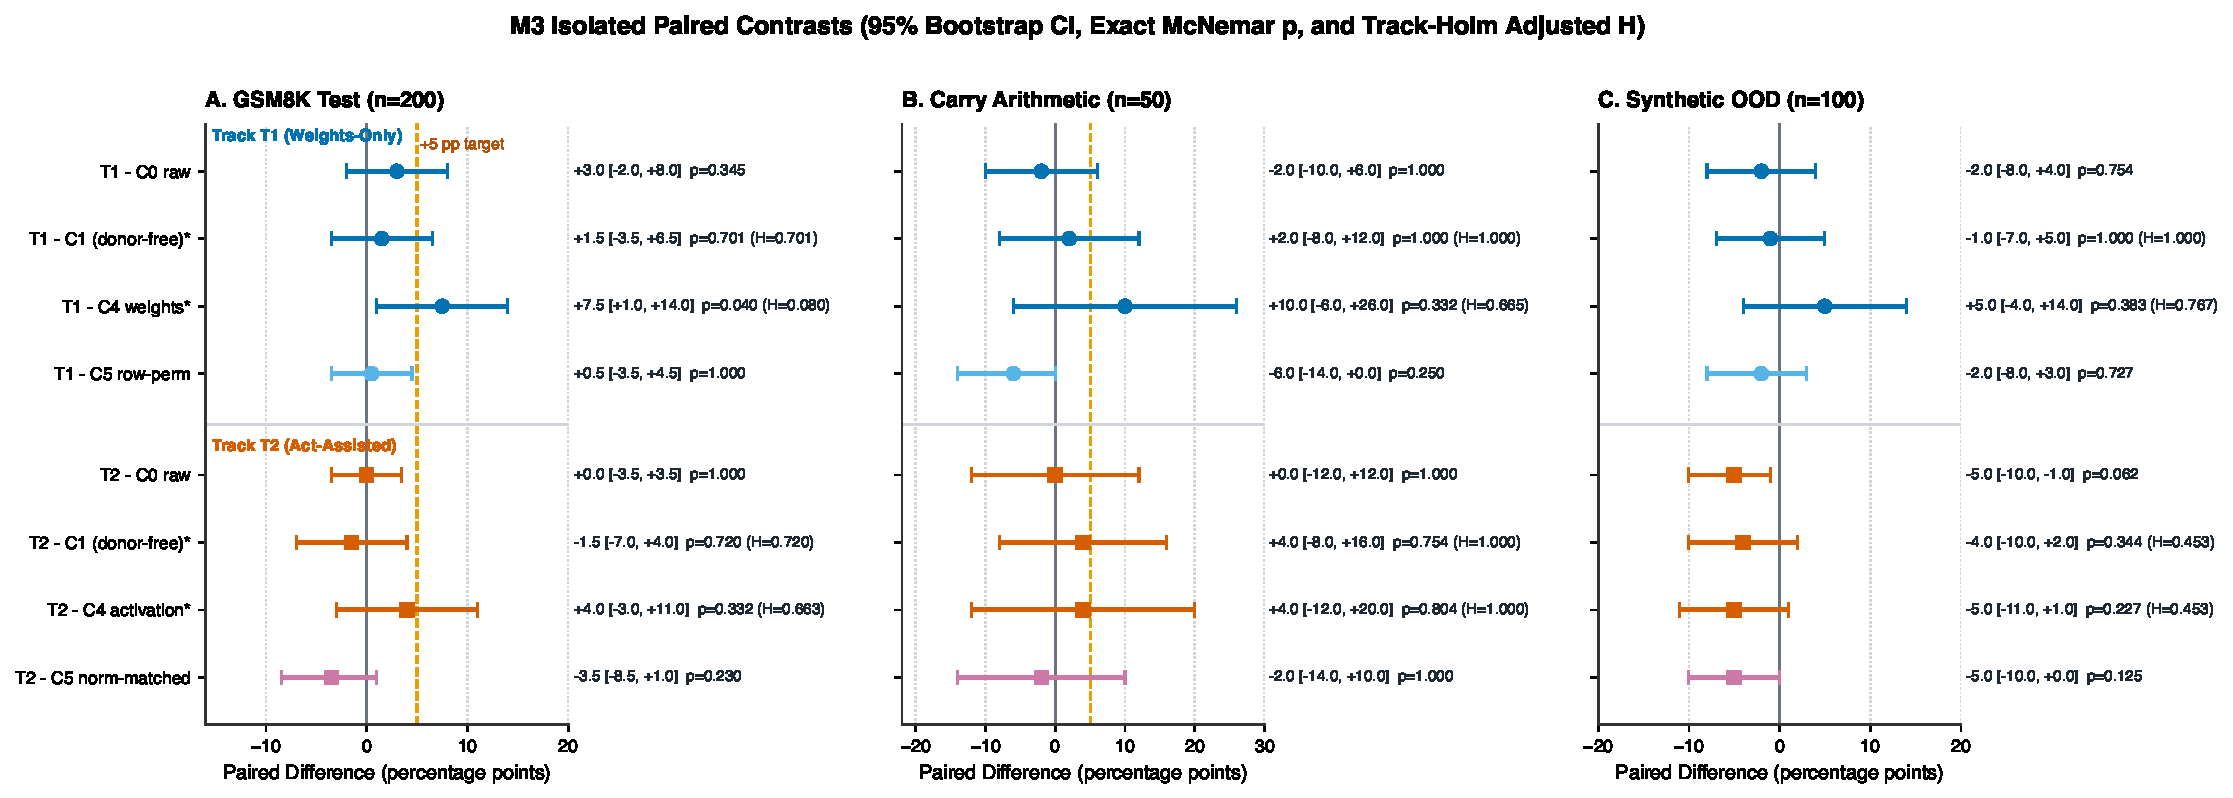
\includegraphics[width=\textwidth]{figures/fig2_m3_forest_contrasts.pdf}
\caption{M3 isolated paired contrasts (95\% bootstrap CIs, exact McNemar $p$, and track Holm-adjusted $H$). Neither track cleared +5.0 pp cleanly or outperformed matched \texttt{C1}, \texttt{C4}, or \texttt{C5} controls.}
\label{fig:forest_contrasts}
\end{figure}

\begin{figure}[htbp]
\centering
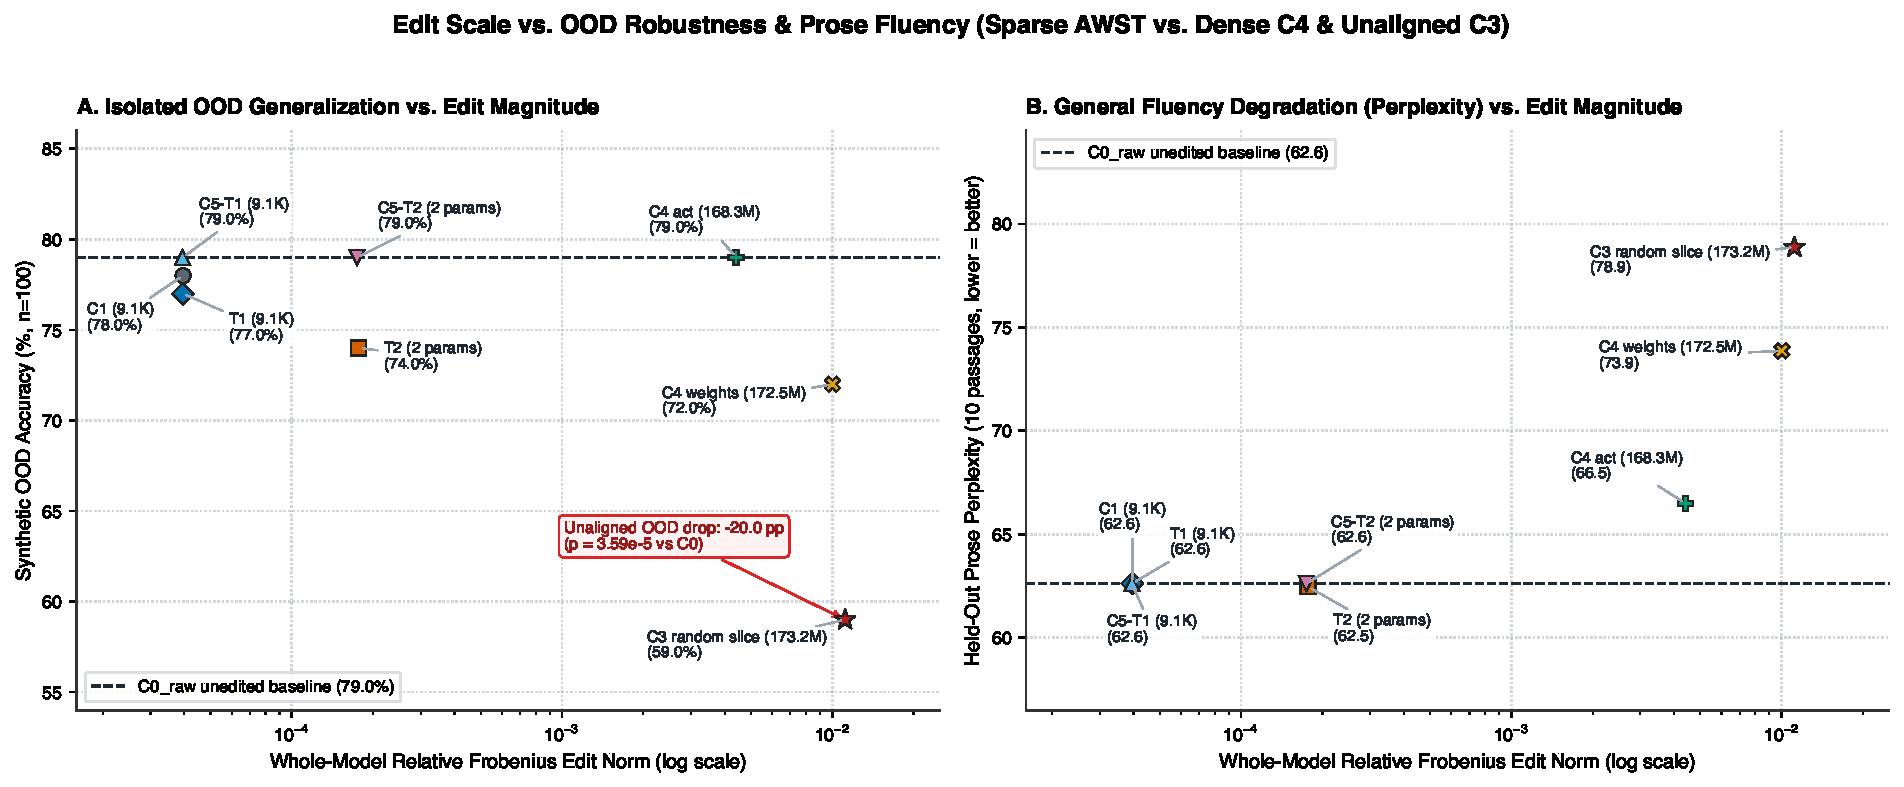
\includegraphics[width=\textwidth]{figures/fig3_edit_magnitude_vs_ood_ppl.pdf}
\caption{Whole-model relative Frobenius edit norm against isolated OOD accuracy (left) and 10-passage prose perplexity (right). Unaligned \texttt{C3} (173.2M entries, \texttt{rel\_frob} $= 1.12\times 10^{-2}$) suffered $-$20.0 pp OOD degradation and +16.24 perplexity rise, while aligned and sparse edits preserved baseline OOD and fluency behavior within noise.}
\label{fig:edit_magnitude}
\end{figure}
\FloatBarrier

\subsection{Joint Preregistered Criteria, Resource Use, and Cost Summary}

\begin{table}[htbp]
\centering
\caption{Evaluation of \texttt{T1} and \texttt{T2} against the preregistered joint feasibility criteria.}
\label{tab:criteria}
\small
\begin{tabularx}{\textwidth}{@{} >{\raggedright\arraybackslash}p{0.31\textwidth} >{\raggedright\arraybackslash}X >{\raggedright\arraybackslash}X @{}}
\toprule
Criterion (Preregistered Freeze) & Track \texttt{T1} (\texttt{H002}) & Track \texttt{T2} (\texttt{H003}) \\
\midrule
Mathematical gain ($\ge +5$ pp GSM8K, $> 0$ carry) & \textbf{Fail}: +3.0 pp [$-$2.0, +8.0]; carry $-$2.0 pp & \textbf{Fail}: 0.0 pp [$-$3.5, +3.5]; carry 0.0 pp \\
Agent \& algorithm advantage ($>$ \texttt{C1}, \texttt{C4}, Holm) & \textbf{Fail}: \texttt{C1} $p=0.701$; \texttt{C4\_weights} Holm $p=0.080$ & \textbf{Fail}: \texttt{C1} $p=0.720$; \texttt{C4\_act} Holm $p=0.663$ \\
Donor dependence ($>$ \texttt{C5} \& reversion) & \textbf{Fail}: +0.5 pp [$-$3.5, +4.5] vs.\ \texttt{C5\_T1} & \textbf{Fail}: $-$3.5 pp [$-$8.5, +1.0] vs.\ \texttt{C5\_T2} \\
Generalization (\texttt{synthetic\_ood\_test}) & \textbf{Fail}: $-$2.0 pp [$-$8.0, +4.0] & \textbf{Fail}: $-$5.0 pp [$-$10.0, $-$1.0] ($p=0.0625$) \\
Capability retention (\texttt{ret\_ifeval} $\le 3$ pp loss) & 0.0 pp (21/30 identical; sparse caveat) & 0.0 pp (21/30 identical; sparse caveat) \\
Structural invariants (0 grad, 153/153 vision) & \textbf{Pass}: 873,438,784 params; 0 grad steps & \textbf{Pass}: 873,438,784 params; 0 grad steps \\
Device efficiency ($\le 10\%$ of \texttt{C0\_raw} 106.5 tok/s) & 100.9 tok/s (0.947$\times$); 2395.8 MB post-eval MPS & 101.4 tok/s (0.952$\times$); 2395.8 MB post-eval MPS \\
\bottomrule
\end{tabularx}
\end{table}

Across all milestones (M0--M4), local execution on M4 Max consumed \textbf{\$0.00 in direct paid API or cloud GPU charges} against the \$200.00 study ceiling and kept local storage at \textbf{18 GB} ($< 30$ GB cap) (Table~\ref{tab:criteria}). Codex subscription usage (\texttt{GPT-6.2 Astra}, shadow-billed at live API rates of \$8/\$0.40/\$40 per million uncached input / cached input / output+reasoning tokens) totaled \textbf{\$14.2912} within the \$20.00 authorized M2 pilot gate: \texttt{H001} (\$1.1003), \texttt{H002} (\$6.0415), \texttt{H003} (\$5.9884), and \texttt{H004} (\$1.1610). Notice that \texttt{H002} (\$6.0415) + \texttt{H003} (\$5.9884) = \$12.0300, exceeding the initial \$12.00 Astra pilot sub-allocation by \$0.0300, which was transparently reconciled against the approved \$3.00 contingency inside \texttt{D005}.

\section{Analysis and Audit Reconciliation}

Independent arithmetic and methodology review (\texttt{H004}, \codepath{runs/codex_h004/review.md}) highlighted seven interpretive constraints that qualify what these measurements establish.

\subsection{Why Did \texttt{T1} and \texttt{T2} Fail to Transfer Mathematical Reasoning?}

\begin{enumerate}
\item \textbf{Shallow Input-Layer Anchoring (\texttt{T1}) vs.\ Distributed Arithmetic Computation:} Consistent with Goworek et al.'s~\cite{goworek2026replicating} observation that LLM programmers disproportionately anchor on input/embedding layers when donor activations are forbidden, \texttt{H002} localized the entire \texttt{T1} intervention to 10 digit token rows (\codepath{embed_tokens.weight}). Multi-digit carry arithmetic and GSM8K word-problem reasoning require multi-step state propagation across middle-to-late DeltaNet, attention, and SwiGLU MLP blocks (layers 8--23), where donor and recipient widths (2048 vs.\ 1024) and representation bases diverge. Nudging digit rows by 1/32 (9,050 entries, \texttt{rel\_frob} $= 3.95\times 10^{-5}$) barely shifted logit margins---fitting noise on development prompts (+4.0 pp GSM8K remainder) that immediately vanished on validation ($-$5.0 pp) and stayed indistinguishable from \texttt{C5\_T1\_rowperm} (+0.5 pp) on test.
\item \textbf{Lack of Causal Necessity in Localized Heads (\texttt{T2}):} In \texttt{H003}, routing correlation (0.9327) and numeric-token RMS selectivity pointed to \codepath{layers.13.linear_attn} head~12, yet ablating that head in the 2B donor slightly \emph{increased} the first-digit logit margin (+0.0208 on GSM8K probes, 0.0 on carry probes). Transplanting two decay scalars (\texttt{A\_log}, \texttt{dt\_bias}) at a non-necessary site reduced OOD accuracy (0 gains, 5 losses, $-$5.0 pp [$-$10.0, $-$1.0]) and trailed \texttt{C5\_T2\_norm\_matched} ($-$3.5 pp).
\item \textbf{The Perturbation Scale Chasm (Ultra-Sparse Agent Edits vs.\ Dense Alignment):} Comparing \texttt{T1}/\texttt{T2} against \texttt{C4} reveals an extreme gap in intervention footprint: the agent edited 9,050 (0.0010\%) or 2 ($2.3\times 10^{-7}$\%) parameters (\texttt{rel\_frob} $\le 1.77\times 10^{-4}$), avoiding collateral fluency damage (\texttt{prose\_ppl} 62.47--62.62 vs.\ 62.63), whereas algorithmic baselines \texttt{C4\_weights}/\texttt{C4\_act} edited 168M--172M parameters ($\sim 19\%$ of the model, \texttt{rel\_frob} $= 4.4\times 10^{-3}$ to $1.0\times 10^{-2}$) and degraded GSM8K ($-$4.5 pp, $-$4.0 pp) and perplexity (73.86, 66.50). Standard ERM \texttt{Qwen3.5-0.8B} weights~\cite{ropinski2026editready} appear too distributed and coupled for either 2-scalar surgical edits or naive 16-layer linear projections to unlock 2B reasoning cleanly without gradient adaptation.
\end{enumerate}

\subsection{Statistical Power, Discordance, and \texttt{T1} vs.\ \texttt{T2} Precision}

Our $n=200$ \texttt{gsm8k\_test} subset was frozen prior to isolated evaluation (\texttt{D011}) for local runtime feasibility without a prospective formal power calculation. Sensitivity integration over the binomial discordant count shows that at $n=200$ pairs and a true +5.0 pp effect, two-sided exact McNemar attains roughly 40\% power at $\alpha=0.05$ (30\% at $\alpha=0.025$) under 14\% discordance (\texttt{T1} $-$ \texttt{C0} observed 28/200), and 26\% (18\% at $\alpha=0.025$) under 23.5\% discordance (\texttt{T1} $-$ \texttt{C4\_weights} observed 47/200). Crucially, \textbf{\texttt{T1} $-$ \texttt{C0\_raw} (+3.0 pp [$-$2.0, +8.0]) still spans the +5.0 pp planning target} while failing Holm and \texttt{C5} joint criteria, whereas \textbf{\texttt{T2} $-$ \texttt{C0\_raw} (0.0 pp [$-$3.5, +3.5]) excludes +5.0 pp} on these 200 items. Neither interval captures session-to-session editing variance because $N=1$ agent session ran per track. Moreover, when discordant flips are very sparse---such as \texttt{T2} losing 5 OOD items with 0 gains---percentile bootstrap intervals exclude zero ([$-$10.0, $-$1.0]) even when exact two-sided McNemar remains above 0.05 ($p = 0.0625$); reporting both prevents over-interpreting sparse-flip CIs.

\subsection{Fair Decomposition and Control Asymmetries}

The near-threshold contrast \texttt{T1} $-$ \texttt{C4\_weights} (+7.5 pp [+1.0, +14.0], raw $p = 0.040$, Holm $p = 0.080$) splits into +3.0 pp (\texttt{T1} $-$ \texttt{C0\_raw}) plus $-$4.5 pp (\texttt{C4\_weights} $-$ \texttt{C0\_raw}, [$-$11.5, +2.5], $p = 0.272$). Attributing that gap solely to \texttt{C4\_weights} degradation or claiming \texttt{T1} superiority overstates the data. Likewise, control symmetry is incomplete across design axes: \texttt{C1} matched \texttt{T1}'s 10 digit rows cleanly, but no donor-free counterpart searched \codepath{layers.13.linear_attn} to match \texttt{T2}'s head-selection search; \texttt{C2} served as a validation-only noise check; \texttt{C4} touched $\sim 10^{4}\times$--$10^{8}\times$ more parameters than \texttt{T1}/\texttt{T2}; and \texttt{C5} used one random seed (\texttt{seed=42}), with \texttt{C5\_T2\_norm\_matched} testing donor direction conditional on \texttt{T2}'s activation-selected head and offset rather than random head selection.

\subsection{Procedural Isolation vs.\ Benchmark Novelty, Parsing, Retention, and Efficiency}

\begin{enumerate}
\item \textbf{Isolation vs.\ Exposure:} Freeze commit \texttt{d12e8fb} preceded isolated execution (\texttt{42b859b}), verifying dataset digests and external log storage (\codepath{/Users/kaiwendu/.awst_isolated_eval/m3_logs/}). However, \texttt{Qwen3.5}'s pretraining exposure to public GSM8K is unknown, and our synthetic generator/6 OOD wording templates (\codepath{src/data/synthetic_arithmetic.py}) are agent-readable, testing novel two-step phrasings rather than unseen carry algorithms.
\item \textbf{Parser and \textbf{H2} Attribution:} Across M3 GSM8K, \texttt{C0\_raw}, \texttt{T1}, and \texttt{T2} logged 0.0\% unparseable outputs, 10.5\% / 10.0\% / 10.0\% truncations ($\ge 1024$ tokens), and 3.5\% / 5.0\% / 4.5\% loop flags. Because \texttt{parser.py} falls back to the last extracted numeric token on truncated generations and M3 aggregates do not break down correctness by extraction tier or include a blinded human audit, numeric agreement alone cannot isolate mathematical reasoning from completion shifts (\textbf{H2}).
\item \textbf{Secondary \textbf{H3} Scope:} \texttt{C3} failed sharply on OOD ($-$20.0 pp, $p = 3.59\times 10^{-5}$) and 10 prose passages (62.63 $\rightarrow$ 78.87), with \texttt{C4\_weights} serving as its closest same-layer, same-$\alpha=0.05$ comparator (+13.0 pp OOD, raw $p = 0.0192$, though $-$2.5 pp on GSM8K). Because selection, SVD projection, and Hungarian neuron matching changed together across one \texttt{C3} draw (\texttt{seed=42}), \textbf{H3} shows specific OOD sensitivity to unaligned MLP copying rather than isolating alignment as a sole causal mechanism or establishing broad prose fluency.
\item \textbf{Retention and Device Efficiency Bounds:} On the 30-item format suite, \texttt{C0\_raw}, \texttt{T1}, and \texttt{T2} passed the exact same 21/30 items; one discordant flip equals 3.33 pp, so a zero-discordance bootstrap CI of [0, 0] reflects discreteness rather than certifying population loss $< 3$ pp across general capabilities. Similarly, \texttt{peak\_mps\_allocated\_mb} (2395.8 MB) sampled driver allocation once post-evaluation rather than tracking mid-generation peaks, \texttt{peak\_rss\_mb} reflected process-lifetime maxima (744--12,240 MB across multi-arm subprocess order), and tokenizer/runtime-graph equality was attested directly during M2 verification (\texttt{verify\_h002.py}, \texttt{verify\_h003.py}) rather than re-hashed inside M3.
\end{enumerate}

\section{Limitations, Safety, Licensing, and Future Work}

\paragraph{Key Limitations.}
First, Stages~2 (\codepath{Qwen/Qwen3.5-9B}), 3 (\codepath{google/gemma-4-E2B-it}), and 4 (\codepath{moonshotai/Kimi-K3.1-Pro}) were skipped after verified negative Stage~1 validation (\texttt{D011}), leaving larger donors, cross-family transfer, and remote trillion-parameter transplantation (\textbf{H4} downstream efficacy) untested. Second, each track ran a single agent session ($N=1$) instead of $\ge 5$ independent sessions, precluding estimates of cross-session variance. Third, all evaluations used \texttt{enable\_thinking=False} at 1,024 tokens; thinking-mode transfer under vLLM \texttt{presence\_penalty=1.5} and 32K context was not attempted.

\paragraph{Safety and Licensing.}
All evaluated checkpoints carry permissive Apache~2.0 licenses, no unapproved model weights were downloaded or uploaded, zero hidden test strings entered version control, and zero safety guardrails were weakened (\texttt{ret\_ifeval} non-math constraints held unchanged).

\paragraph{Future Work.}
Promising next directions include: (1) investigating the intermediate regime between 2-scalar edits and 170M-parameter dense projection---for example, low-rank subspace or multi-layer MLP/attention circuit grafting conditioned on positive causal ablation necessity; (2) pretraining or adapting small recipients with \emph{Edit-Ready} objectives~\cite{ropinski2026editready}; (3) running $\ge 5$ independent multi-session replicates with prospective discordant-rate power calculations; and (4) hardening frozen evaluators to enforce unique identical ID assertions, cryptographic log-to-manifest binding, and parse-method-stratified audits (\texttt{H004} recommendations).

\section{Conclusion}

Returning directly to our six research questions based on verified M0--M4 evidence:
\begin{enumerate}
\item \textbf{RQ1 \& H1 (Primary AWST Feasibility):} Within Stage~1 (\codepath{Qwen/Qwen3.5-2B} $\rightarrow$ \codepath{Qwen/Qwen3.5-0.8B}, \texttt{nothink 1024}, $N=1$ session/track), neither frozen weights-only (\texttt{T1}) nor activation-assisted (\texttt{T2}) transplantation met the preregistered joint success criteria. \texttt{T1} (+3.0 pp [$-$2.0, +8.0] vs.\ \texttt{C0\_raw}, carry $-$2.0 pp) remains inconclusive on absolute GSM8K effect size while failing Holm-adjusted superiority (\texttt{C1}, \texttt{C4\_weights}) and donor dependence (\texttt{C5\_T1}), whereas \texttt{T2} (0.0 pp [$-$3.5, +3.5] vs.\ \texttt{C0\_raw}, $-$5.0 pp OOD) produced a clear negative outcome on these evaluated checkpoints.
\item \textbf{RQ2 \& RQ3 (Agent vs.\ Conventional \& Donor-Free Controls):} Neither \texttt{T1} nor \texttt{T2} established statistically reliable advantages over donor-free \texttt{C1} (+1.5 pp, $-$1.5 pp), algorithmic \texttt{C4} after Holm correction ($p = 0.080$, $p = 0.663$), or shuffled-donor \texttt{C5} (+0.5 pp, $-$3.5 pp). Conversely, dense algorithmic transfer (\texttt{C4\_weights}, \texttt{C4\_act}) regressed on GSM8K ($-$4.5 pp, $-$4.0 pp) and prose perplexity (73.86, 66.50), exposing a severe sparsity-vs.-disruption trade-off.
\item \textbf{RQ4 \& H2/H3 (Generalization and Alignment):} Stage~3 cross-family transfer (\texttt{RQ4}) was gated and skipped (\texttt{D011}). Generalization (\textbf{H2}) failed for both \texttt{T1} ($-$2.0 pp OOD) and \texttt{T2} ($-$5.0 pp OOD). On \textbf{H3}, unaligned slice copying (\texttt{C3}) failed sharply on unseen OOD templates ($-$20.0 pp, $p = 3.59\times 10^{-5}$) and prose perplexity (78.87), which aligned \texttt{C4\_weights}/\texttt{C4\_act} and sparse edits avoided.
\item \textbf{RQ5 \& H4 (Selective Remote Access):} Byte-range HTTP 206 retrieval (9,892.98$\times$ reduction, 176,584 B read vs.\ 1.75 GB shard) is technically reliable and bit-exact, though downstream cross-scale transfer efficacy using remote donor slices remains unproven.
\item \textbf{RQ6 (Competency vs.\ Real-LLM Transfer):} Toy synthetic network competency (3/3 for both \texttt{Gemini 4 Neon} and \texttt{GPT-6.2 Astra}) did not predict successful cross-scale LLM circuit transplantation, underscoring the necessity of rigorous held-out validation and shuffled-donor controls.
\end{enumerate}

\bibliographystyle{plainnat}
\bibliography{references}

\appendix

\section{Pinned Reproducibility Registry}

\begin{itemize}
\item \textbf{Base Recipient (\codepath{Qwen/Qwen3.5-0.8B}):} revision \codehash{2fc06364715b967f1860aea9cf38778875588b17}, primary shard \codepath{model.safetensors-00001-of-00001.safetensors}, SHA-256 \codehash{04b1c301231dd422b8860db31311ab2721511346a32cb1e079c4c4e5f1fe4696}, 873,438,784 stored / 852,985,920 active runtime params (153 frozen vision tensors $=$ 100,592,896 params).
\item \textbf{Donor (\codepath{Qwen/Qwen3.5-2B}):} revision \codehash{15852e8c16360a2fea060d615a32b45270f8a8fc}, primary shard SHA-256 \codehash{aa33250c4fc64891ddfaba3a314fd9542ea371843c387178b425fbcc5ed680b1}, 2,274,069,824 stored params.
\item \textbf{Persistent Finalist Shard Digests (\codepath{runs/manifests/m3_frozen_checkpoint_audit.json}):}
  \texttt{C1}: \codehash{b11f16df6de7bfb5f060789477a4e67764946f111feccd3a871d2440227ad11a};
  \texttt{T1}: \codehash{da9ad05f9c4931477197b46581ed83653485f16763eeb7197bb9aaead2f81414};
  \texttt{T2}: \codehash{ea5c744fe4d6627c2faefee13e2c2ad97c44f3ad012c7adc491d60290f6bb732};
  \texttt{C4\_weights}: \codehash{1ecd31aab734047054734dd4ffb3ad7a97f1464cb92531d0d23419928fa0fc8d};
  \texttt{C4\_act}: \codehash{2814219eb02445e4e74afad31d38fb0f8536be93d07b597dd2444698b6792491}.
\item \textbf{Dataset Digests (\codepath{data/dataset_manifest.json}):} \texttt{synthetic\_dev} (900, \texttt{c2e41927...}), \texttt{synthetic\_val} (300, \texttt{cd5e3b7f...}), \texttt{gsm8k\_dev} (500, \texttt{6e2fbfa1...}), \texttt{gsm8k\_val} (200, \texttt{4aa4ef28...}); external isolated \codepath{/Users/kaiwendu/.awst_isolated_eval/}: \texttt{synthetic\_test} (300, \texttt{c81c7414...}), \texttt{synthetic\_ood\_test} (100, \texttt{4904d73b...}), \texttt{gsm8k\_test} (1,319, \texttt{5315f256...}, M3 sampled $n=200$ via \texttt{Random(20261126)}).
\end{itemize}

\section{Frozen Prompt and Key Codex Handoff Manifests}

\begin{itemize}
\item \textbf{Math Prompt (\codepath{src/evaluation/runner.py}):} User prompt embeds each problem verbatim with a single deterministic final-answer formatting instruction inside the \texttt{Qwen3.5} chat template rendered with \texttt{enable\_thinking=False}, decoded greedily (\texttt{do\_sample=False}, \texttt{max\_new\_tokens=1024}, \texttt{bfloat16}, batch size~1 on MPS).
\item \textbf{Handoffs \& Verification Artifacts:}
  \codepath{docs/handoffs/H001_rq6_competency_pilot.md},
  \codepath{docs/handoffs/H002_stage1_awst_t1.md},
  \codepath{docs/handoffs/H003_stage1_awst_t2.md},
  \codepath{docs/handoffs/H004_m3_independent_review.md};
  Antigravity independent reports
  \codepath{results/m1_stage0_baselines.json},
  \codepath{results/m1_remote_reader_validation.json},
  \codepath{results/m2_rq6_competency_comparison.json},
  \codepath{results/m2_conventional_baselines.json},
  \codepath{results/m2_h002_verification.json},
  \codepath{results/m2_h003_verification.json},
  \codepath{results/m3_isolated_evaluation.json};
  Codex reports
  \codepath{runs/competency_astra/report.md},
  \codepath{runs/codex_h002/report.md},
  \codepath{runs/codex_h003/report.md},
  \codepath{runs/codex_h004/review.md}.
\end{itemize}

\end{document}
